\documentclass[12pt]{standalone}
\usepackage{tikz}
\usetikzlibrary{positioning}
\begin{document}
\large
\pagestyle{empty}
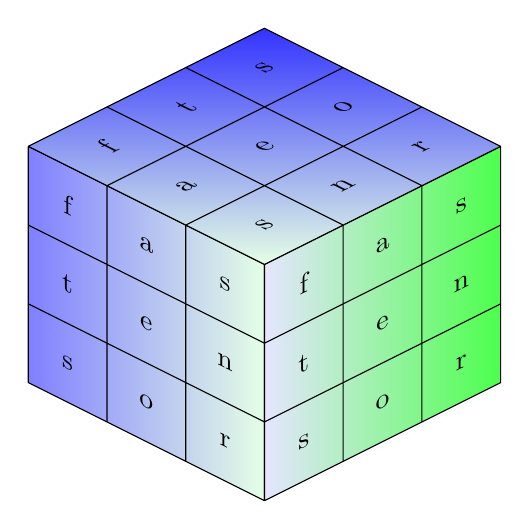
\begin{tikzpicture}[every node/.style={minimum size=1cm},on grid]
\begin{scope}[every node/.append style={yslant=-0.5},yslant=-0.5]
  \shade[right color=green!10, left color=blue!50] (0,0) rectangle +(3,3);
  \node at (0.5,2.5) {f};
  \node at (1.5,2.5) {a};
  \node at (2.5,2.5) {s};
  \node at (0.5,1.5) {t};
  \node at (1.5,1.5) {e};
  \node at (2.5,1.5) {n};
  \node at (0.5,0.5) {s};
  \node at (1.5,0.5) {o};
  \node at (2.5,0.5) {r};
  \draw (0,0) grid (3,3);
\end{scope}
\begin{scope}[every node/.append style={yslant=0.5},yslant=0.5]
  \shade[right color=green!70,left color=blue!10] (3,-3) rectangle +(3,3);
  \node at (3.5,-0.5) {f};
  \node at (4.5,-0.5) {a};
  \node at (5.5,-0.5) {s};
  \node at (3.5,-1.5) {t};
  \node at (4.5,-1.5) {e};
  \node at (5.5,-1.5) {n};
  \node at (3.5,-2.5) {s};
  \node at (4.5,-2.5) {o};
  \node at (5.5,-2.5) {r};
  \draw (3,-3) grid (6,0);
\end{scope}
\begin{scope}[every node/.append style={yslant=0.5,xslant=-1},yslant=0.5,xslant=-1]
  \shade[bottom color=green!10, top color=blue!80] (6,3) rectangle +(-3,-3);
  \node at (3.5,2.5) {f};
  \node at (3.5,1.5) {a};
  \node at (3.5,0.5) {s};
  \node at (4.5,2.5) {t};
  \node at (4.5,1.5) {e};
  \node at (4.5,0.5) {n};
  \node at (5.5,2.5) {s};
  \node at (5.5,1.5) {o};
  \node at (5.5,0.5) {r};
  \draw (3,0) grid (6,3);
\end{scope}
\end{tikzpicture}
\end{document}